%!TEX root = ../main.tex
% chktex-file 13

\subsection{AREPO}\label{sec:arepo}
Arepo is a massively parallel astrophysics code for the simulation of gravitational N-body systems and magnetohydrodynamics, both on Newtonian as well as cosmological backgrounds.
There are a number of versions in the community, originating from a common closed-source code base.
A version with reduced functionality was made publicly available under GPLv3\cite{weinberger_arepo_2020, springel_arepo_nodate}.
Different research groups use code bases derived from the closed source version, including the Sijaki group at the University of Cambridge.
This code~\cite{sijaki_arepo_nodate}, which was part of the DiRAC3 procurement, acceptance testing and technical commissioning, forms the basis of porting efforts to be undertaken within the course of this project.

In Arepo, the computational domain is discretized using a fully adaptive, dynamic unstructured Voronoi mesh, which is moving with the fluid in a quasi-Lagrangian way and that is paired with a finite volume approach for the hydrodynamics.
Arepo is written in C, parallelized with MPI and some of the code bases, including the one used in this project, have additionally OpenMP shared memory parallelization.
To the best of our knowledge, there is currently no version of this code that can target accelerators with any of the computational kernels in the main time loop.
As a C application that includes already OpenMP parallelization, we intend to follow Intel's recommendation to use OpenMP 5 offloading to target GPUs.

% In order to run simulations efficiently on the next generation of supercomputers there are a few key aspects that need to be taken into account.
% Some of those steps are already well known in the HPC community for years, i.e. well balanced computational load or the avoiding collective communication as much as possible.
% Apart from that it will be increasingly important to make use of hybrid architectures, i.e. accelerators.
In contrast to codes described above, where suitable kernels for GPU execution have already been identified in prior porting efforts, this selection process has to be done as an additional first step for this purely CPU-based code.
Therefore, extensive profiling of the code base has been undertaken using one of the test cases that are also used to verify code correctness to analyze the potential of porting parts of Arepo to GPUs.
Hence, a first analysis was carried out using Intel VTune profiler and Intel Trace Analyzer, producing two key insights:

The first insight was that a significant share of the overall run time is spent waiting in a synchronisation step that uses global MPI communication.
The purpose of this step is to detect the need for program interruption to trigger saving the current state in a snapshot file and termination of the program.
Since there is no data dependence on this communication step, it is possible to reverse the logic of this routine, replace the respective MPI calls with their non-blocking counterparts and trigger the snapshot writing after the next time step.
This enables perfect overlap of computation and communication at the expense of a one time step lag in the snapshot writing.
Even on this small single-node test case this already reduces the run time of the main time loop by 2\%, promising even larger savings in production runs that use significantly more nodes.

\begin{figure}[htp]
	\centering
	\subfloat{ 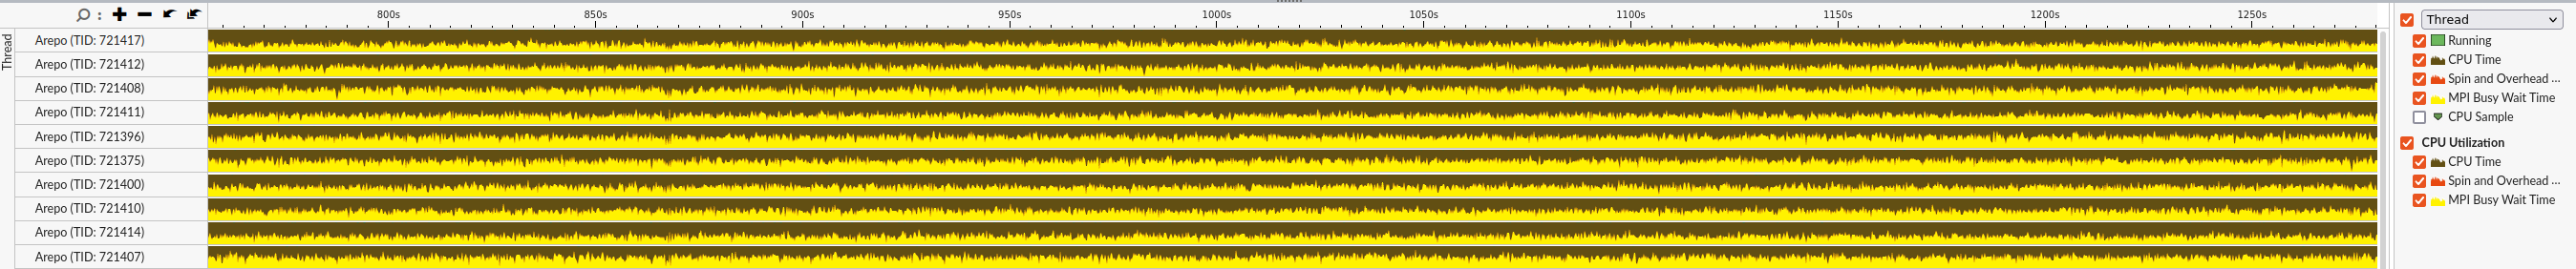
\includegraphics[clip,width=\textwidth]{arepo_blocking.png}}
	\subfloat{ 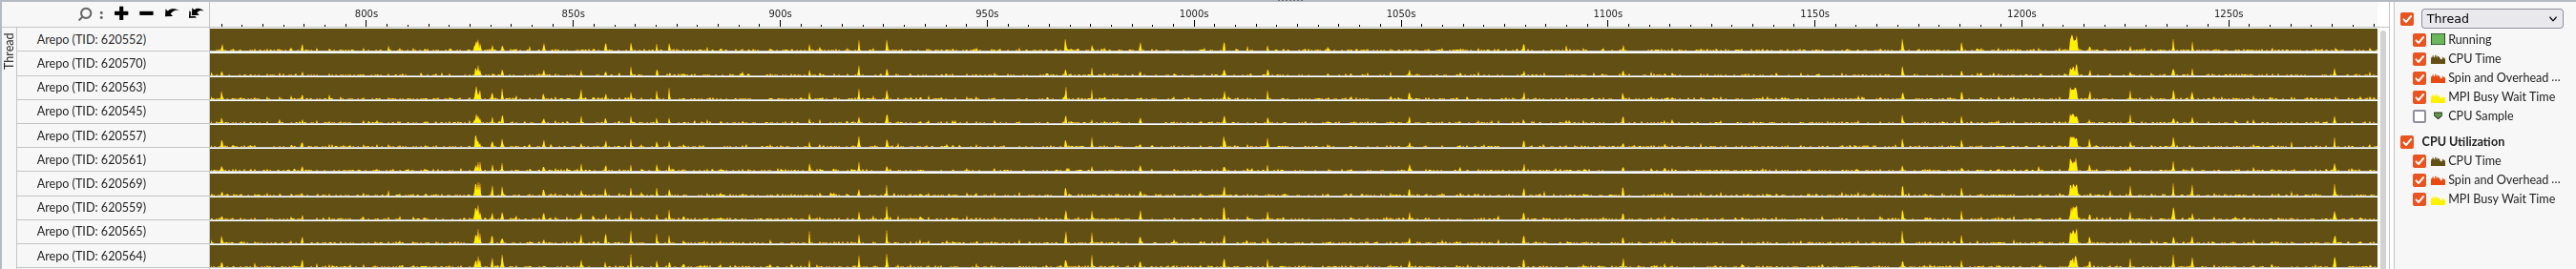
\includegraphics[clip,width=\textwidth]{arepo_nonblocking.png}}
	\caption{Significant reduction of MPI Busy Wait Time (yellow) in the lower VTune Profiler graphic compared to the top version where blocking communication was used. Shown for a random selection of ranks}
	\label{fig:arepo_mpicom} % chktex 24
\end{figure}

Second profiling outcome and original motivation for this analysis was to understand the distribution of run time across the different parts of a time step and subsequently to identify suitable candidates for GPU porting.
The two most time-consuming parts proved to be the evaluation of gravitational forces, which is carried out in two half steps at the beginning and end of a time step, and the creation of the Voronoi mesh in-between.

The next step in the analysis was to use Intel's Offload Advisor to see if these contain any kernels that would readily benefit from GPU offloading.
However, with the current structure of the underlying algorithm the Offload Advisor judged every routine to suffer from too much overhead when ported to GPU.
Only relatively short loops within sub steps of the mesh creation routines were classified as offload candidates that could potentially see any speed-up.

Overall, this suggests that for a successful GPU port of Arepo it may not be sufficient to port few individual kernels to achieve performance gains but requires a better understanding of the numerical method and possibly adaptation of the algorithm to better map to the target hardware.
For that, we are in active discussions with the developers at the University of Cambridge and take into account prior experience and publications in the scientific domain.

%\begin{itemize}
%    \item reference to paper to port
%    \item https://arxiv.org/abs/1610.07279
%    \item https://arxiv.org/abs/0907.3390
%    \item https://arxiv.org/abs/1909.07439
%\end{itemize}
